\documentclass[12pt]{article}


\usepackage{graphicx}
\usepackage{anysize}
\usepackage[spanish]{babel}
\marginsize{1cm}{3cm}{0cm}{0cm}


\usepackage{eso-pic}
\newcommand\BackgroundPic{
\put(0,0){
\parbox[b][\paperheight]{\paperwidth}{%
\vfill
\centering
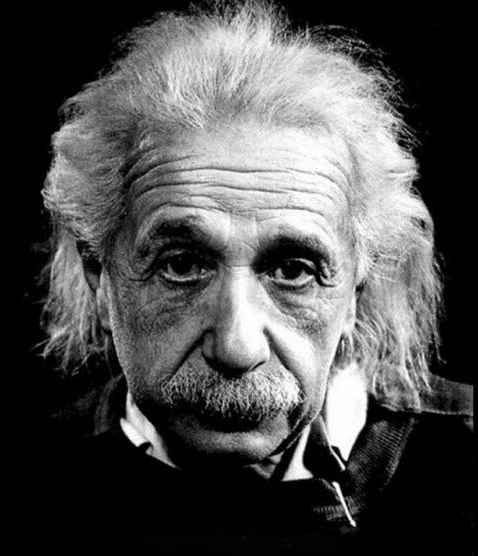
\includegraphics[width=\paperwidth,height=\paperheight,
keepaspectratio]{eisten.png}%
\vfill
}}}


\begin{document}
\AddToShipoutPicture*{\BackgroundPic}
\pagestyle{empty}
\begin{figure}[ht]
\begin{minipage}{0.3 \textwidth}
\begin{center}
\textbf{INGENIERIA}
\end{center}
El dise\~no de una turbina requiere de colaboraci\'on de ingenieros de diversas ramas. Los ingenieros de cada especializaci\'on deben tener 
conocimientos básicos de otras \'areas afines para resolver problemas complejos y de disciplinas interrelacionadas.
La ingenier\'ia es el conjunto de conocimientos y t\'ecnicas científicas aplicadas a la invenci\'on, perfeccionamiento y utilizaci\'on de la 
t\'ecnica industrial en todos sus diversos aspectos incluyendo la resolución de problemas que afectan directamente a los seres humanos en su 
actividad cotidiana.
En ella, el conocimiento, manejo y dominio de las matemáticas, la física y otras ciencias, obtenido mediante estudio, experiencia y práctica, 
se aplica con juicio para desarrollar formas eficientes de utilizar los materiales y las fuerzas de la naturaleza para beneficio de la 
humanidad y del ambiente.
Pese a que la ingeniería como tal (transformación de la idea en realidad) está intrínsecamente ligada al ser humano, su nacimiento 
\end{minipage}
\ \
\hfill \begin{minipage}{0.3 \textwidth}% También se puede indicar en cms
como campo de conocimiento específico está unido al comienzo de la revolución industrial, constituyendo uno de los actuales pilares en el 
desarrollo de las sociedades modernas.
Otro concepto que define a la ingeniería es el saber aplicar los conocimientos científicos a la invención, perfeccionamiento o utilización de 
la técnica en todas sus determinaciones. Esta aplicación se caracteriza por utilizar principalmente el ingenio de una manera más pragmática y 
ágil que el método científico, puesto que una actividad de ingeniería, por lo general, está limitada a un tiempo y recursos dados por 
proyectos. El ingenio implica tener una combinación de sabiduría e inspiración para modelar cualquier sistema en la práctica.


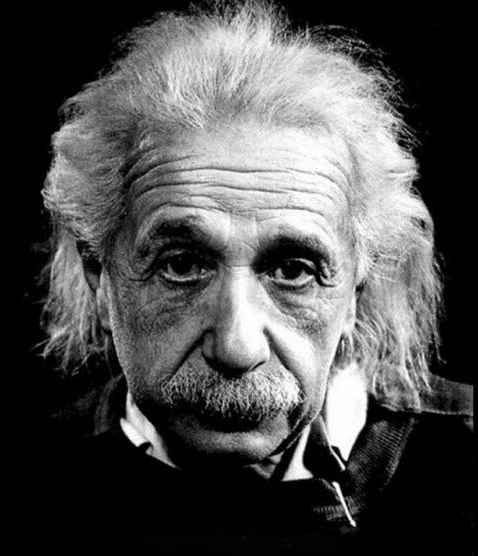
\includegraphics[width=200pt]{eisten.png}
\bigskip
\bigskip


\end{minipage}
\ \
\hfill \begin{minipage}{0.3 \textwidth}% También se puede indicar en cms
\begin{center}
EL INGENIERO
\end{center}
Su función principal es la de realizar diseños o desarrollar soluciones tecnológicas a necesidades sociales, industriales o económicas. Para 
ello el ingeniero debe identificar y comprender los obstáculos más importantes para poder realizar un buen diseño. Algunos de los obstáculos 
son los recursos disponibles, las limitaciones físicas o técnicas, la flexibilidad para futuras modificaciones y adiciones y otros factores 
como el coste, la posibilidad de llevarlo a cabo, las prestaciones y las consideraciones estéticas y comerciales. Mediante la comprensión de 
los obstáculos, los ingenieros deducen cuáles son las mejores soluciones para afrontar las limitaciones encontradas cuando se tiene que 
producir y utilizar un objeto o sistema.
Los ingenieros utilizan el conocimiento de la ciencia y la matemática y la experiencia apropiada para encontrar las mejores soluciones a los 
problemas concretos, creando los modelos matemáticos apropiados de los problemas que les permiten analizarlos rigurosamente y probar las 
soluciones potenciales. 
\end{minipage}
\end{figure}


\end{document}

